\section{Work Definition and Division}
This chapter treats identification and sequencing of activities required during the project and allocation of resources to these activities. As such, it comprises a \gls{wbs} and \gls{wfd} as primary \gls{se} elements to categorize respectively sequence work activities. In addition, the WFD provides interrelations between steps to identify iterations in the work process where appropriate. It is essential that work activities are defined and sequenced in order to allocate resources, as depicted by the Gantt chart.

This chapter is structured as follows. The first section commences with a presentation of the WBS and accompanying discussion to justify the categorization, the second section proceeds with a presentation of the WFD, the third section discusses allocation of resources and presents the Gantt chart. The latter is accompanied by a brief discussion on milestones set to monitor project progress.

\subsection{Work Breakdown Structure}\label{sec:WBS}
Project work has been divided into a number of phases: project planning, literature research, mission analysis, tool development and enhancement, conceptual design of a first set of concepts, detailed design of a number of selected concepts and project close-out. This high-level work division is summarized firstly in the WBS displayed in Figure \ref{fig:wbs}. Whereas the sequence of activities is illustrated by the WFD, the WBS provides a categorization of activities. 

\begin{sidewaysfigure}[ht]
    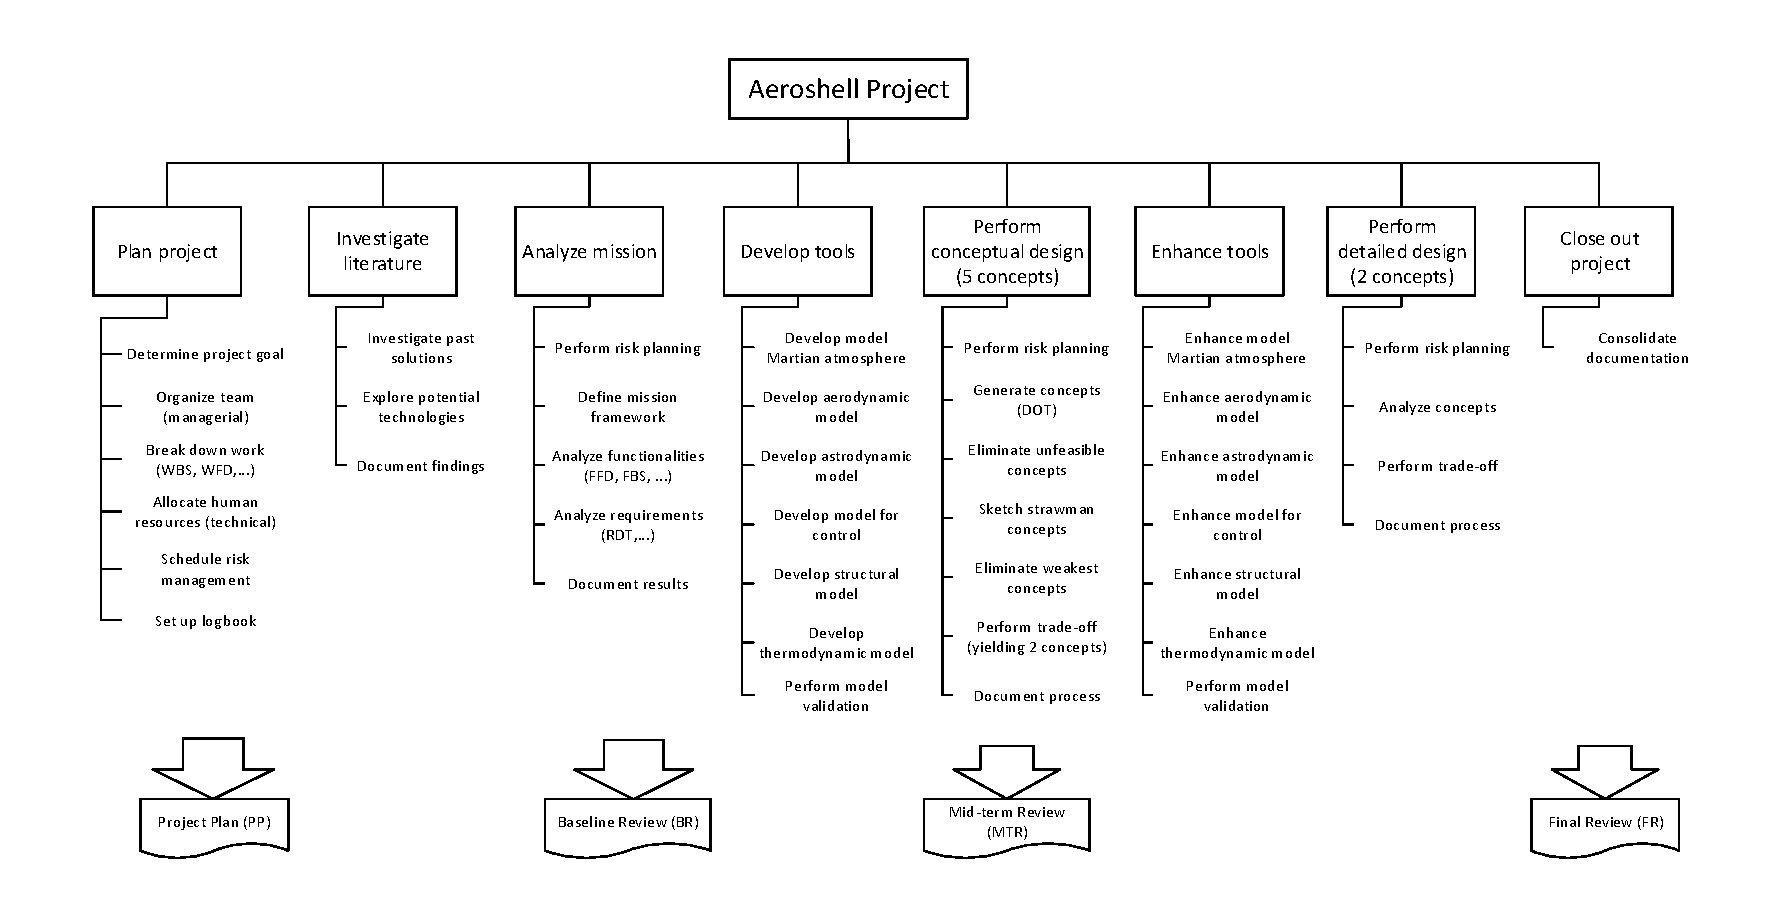
\includegraphics[scale=0.8]{Figure/WBS.pdf}
    \caption{Work Breakdown Structure (WBS) of project.}
    \label{fig:wbs}
\end{sidewaysfigure}

\subsection{Work Flow Diagram}\label{sec:WFD}
The WFD, depicted in Figure \ref{fig:wfd} elaborates on the activities depicted in the WBS (Figure \ref{fig:wbs}) and places them in a sequence. It therefore provides the basis for the allocation of human resources, as done in the Gantt chart, where all sequenced activities are placed in a timeline that fit project constraints in terms of human resources and schedule. Moreover, the WFD provides a graphical means by which to determine activities throughput and to identify iteration loops. 

\begin{sidewaysfigure}[ht]
    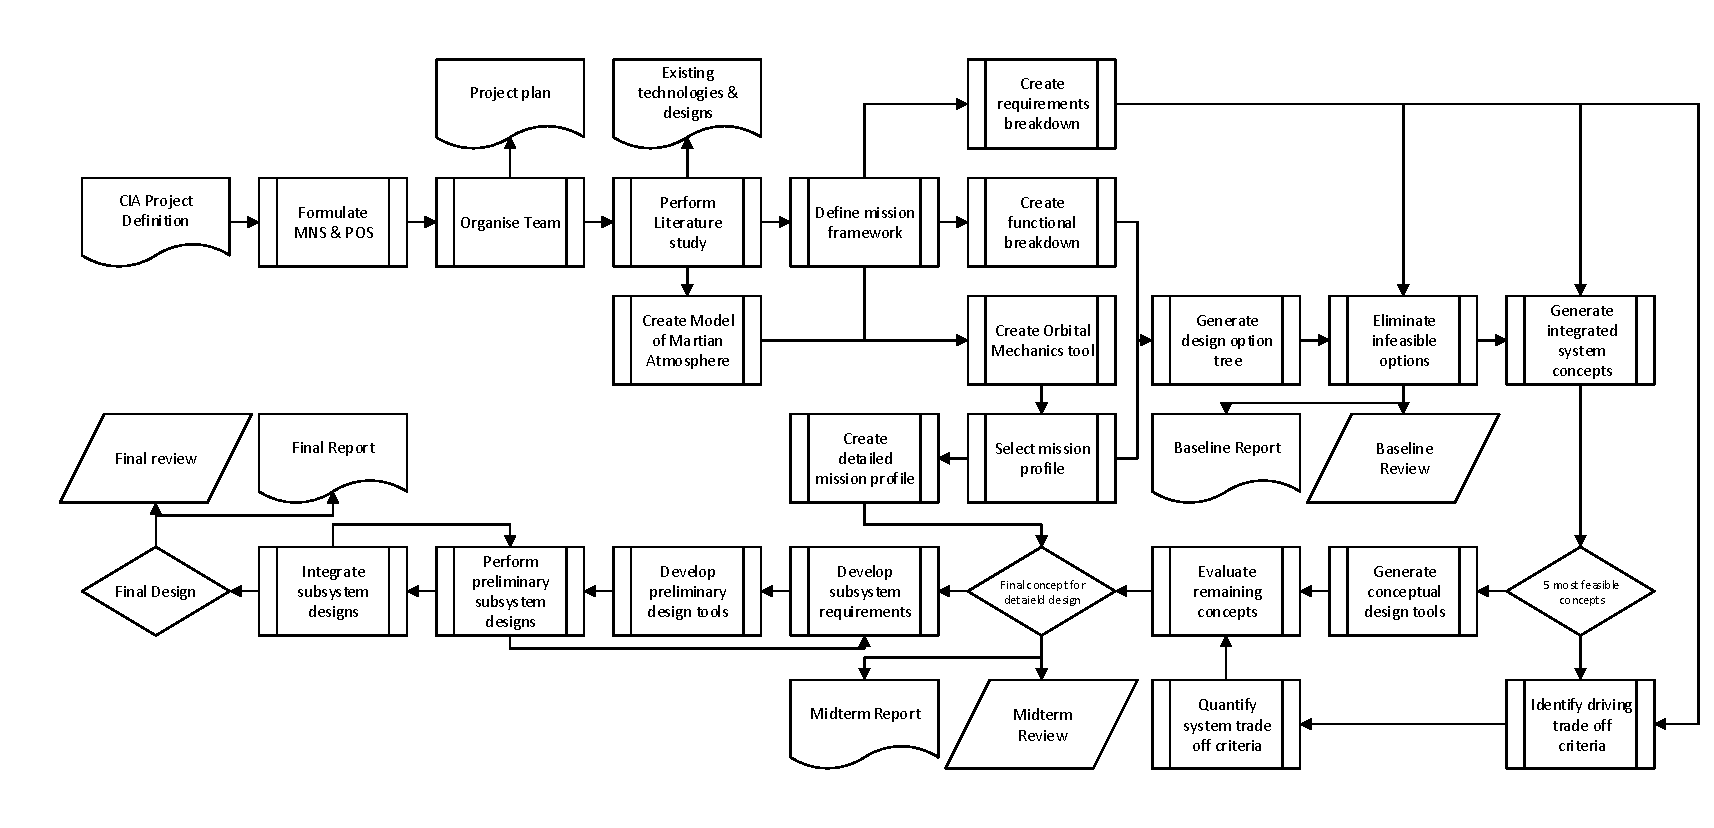
\includegraphics[scale=0.8]{Figure/WFD2.pdf}
    \caption{Work Flow Diagram (WFD) of project.}
    \label{fig:wfd}
\end{sidewaysfigure}

Lastly, it specifies identifiable milestones that close activities and project phases. Predominantly, these milestones are the following:
\begin{itemize}
\item The \gls{pp} finalizes provisional planning of the project, comprising: technical and managerial function appointment to team members, allocation of resources, break-down and sequencing of project work, formulation of a risk management plan and a plan for sustainable development, set-up of archiving, doucmentation and logbook and consolidating a set of project procedures.
\item The \gls{br} (and accompanying Baseline Report) finalize(s) the mission analysis phase by a liaison with the customer for agreement on mission definition, requirements and planning as well as a presentation of initial concepts formulated in the conceptual design phase.
\item The\gls{mtr} (and accompanying Mid-Term Report) finalize(s) the first phase of concept selection, reviewing the concepts for trade-off, the trade-off process and resulting final concepts for further evaluation.
\item \gls{fr} (and accompanying Final Report) finalize(s) the phase of concept selection with a technical presentation and agreement with the customer on the final design and the process by which it was reached. 
\end{itemize}

\subsection{Time Allocation}\label{sec:timeallocation}

A final work structure is given in the planning Gantt chart in which the time allocation for the work packages is displayed. The Gantt chart is given in Figure \ref{fig:GanttChart}, in appendix A, and provides a structured overview of the work to be done, together with allocated time slots and resources. It can be noted that the level of detail decreases as time progresses or milestones are passed. This is in line with the increasing uncertainty about the project outcome. Based on the design choices made around the milestones work to be done differs and resources may be allotted differently. Moreover the organizational breakdown will be altered halfway based on performance so far. Resource allotment is done before the start of each phase. Some work is fixed and is indifferent to design choices made. To this work, typically in the form of required deliverables, time slots have already been allotted in the Gantt Chart. The updating of the Gantt chart based on these design milestones in the different design phases is the work of the planner. This planner function also includes the progress tracking in the Gantt chart as stated in chapter \ref{cha:OBS}.

It should be noted that work is typically allocated to finish a day or more before the milestones. This allows for contingency as well as an optimal functioning of the quality assurance system.



